\newpage
\section{Data}
\label{sec:Data}
\blindtext[1]

Useful package: \texttt{stargazer} produced \vref{tab:summarystats}.
\subsection{Summary Statistics}
\label{sub:Stats}
\blindtext
\begin{kframe}


{\ttfamily\noindent\bfseries\color{errorcolor}{\#\# Error in eval(expr, envir, enclos): konnte Funktion "{}stargazer"{} nicht finden}}\end{kframe}
\blindtext[3]

\subsection{Further Statistics}
\blindtext
\begin{knitrout}
\definecolor{shadecolor}{rgb}{0.969, 0.969, 0.969}\color{fgcolor}\begin{figure}

{\centering 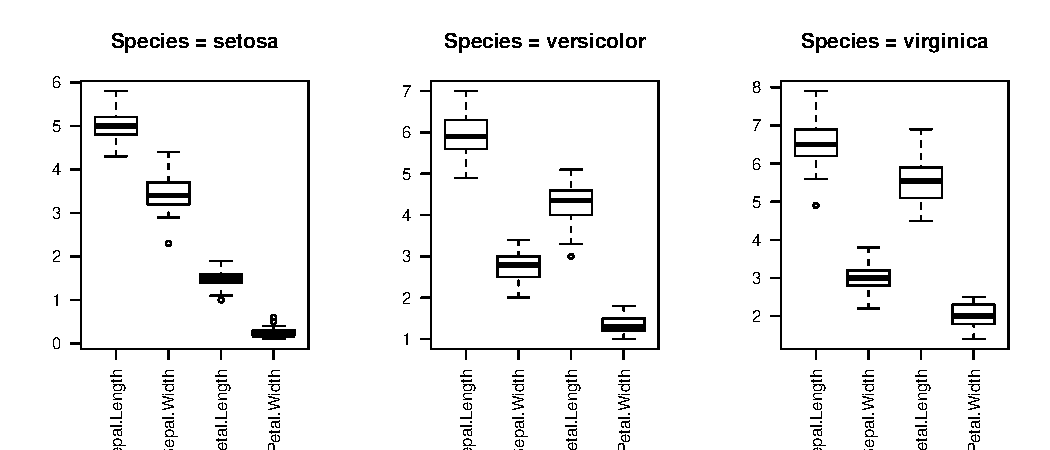
\includegraphics[width=\maxwidth]{figure/boxplots-1} 

}

\caption[Boxplots of the iris data for all three species]{Boxplots of the iris data for all three species}\label{fig:boxplots}
\end{figure}


\end{knitrout}
\blindtext[4]

For the boxplots, see \vref{fig:boxplots}.
